% Options for packages loaded elsewhere
\PassOptionsToPackage{unicode}{hyperref}
\PassOptionsToPackage{hyphens}{url}
%
\documentclass[
]{book}
\usepackage{amsmath,amssymb}
\usepackage{lmodern}
\usepackage{iftex}
\ifPDFTeX
  \usepackage[T1]{fontenc}
  \usepackage[utf8]{inputenc}
  \usepackage{textcomp} % provide euro and other symbols
\else % if luatex or xetex
  \usepackage{unicode-math}
  \defaultfontfeatures{Scale=MatchLowercase}
  \defaultfontfeatures[\rmfamily]{Ligatures=TeX,Scale=1}
\fi
% Use upquote if available, for straight quotes in verbatim environments
\IfFileExists{upquote.sty}{\usepackage{upquote}}{}
\IfFileExists{microtype.sty}{% use microtype if available
  \usepackage[]{microtype}
  \UseMicrotypeSet[protrusion]{basicmath} % disable protrusion for tt fonts
}{}
\makeatletter
\@ifundefined{KOMAClassName}{% if non-KOMA class
  \IfFileExists{parskip.sty}{%
    \usepackage{parskip}
  }{% else
    \setlength{\parindent}{0pt}
    \setlength{\parskip}{6pt plus 2pt minus 1pt}}
}{% if KOMA class
  \KOMAoptions{parskip=half}}
\makeatother
\usepackage{xcolor}
\usepackage{color}
\usepackage{fancyvrb}
\newcommand{\VerbBar}{|}
\newcommand{\VERB}{\Verb[commandchars=\\\{\}]}
\DefineVerbatimEnvironment{Highlighting}{Verbatim}{commandchars=\\\{\}}
% Add ',fontsize=\small' for more characters per line
\usepackage{framed}
\definecolor{shadecolor}{RGB}{248,248,248}
\newenvironment{Shaded}{\begin{snugshade}}{\end{snugshade}}
\newcommand{\AlertTok}[1]{\textcolor[rgb]{0.94,0.16,0.16}{#1}}
\newcommand{\AnnotationTok}[1]{\textcolor[rgb]{0.56,0.35,0.01}{\textbf{\textit{#1}}}}
\newcommand{\AttributeTok}[1]{\textcolor[rgb]{0.77,0.63,0.00}{#1}}
\newcommand{\BaseNTok}[1]{\textcolor[rgb]{0.00,0.00,0.81}{#1}}
\newcommand{\BuiltInTok}[1]{#1}
\newcommand{\CharTok}[1]{\textcolor[rgb]{0.31,0.60,0.02}{#1}}
\newcommand{\CommentTok}[1]{\textcolor[rgb]{0.56,0.35,0.01}{\textit{#1}}}
\newcommand{\CommentVarTok}[1]{\textcolor[rgb]{0.56,0.35,0.01}{\textbf{\textit{#1}}}}
\newcommand{\ConstantTok}[1]{\textcolor[rgb]{0.00,0.00,0.00}{#1}}
\newcommand{\ControlFlowTok}[1]{\textcolor[rgb]{0.13,0.29,0.53}{\textbf{#1}}}
\newcommand{\DataTypeTok}[1]{\textcolor[rgb]{0.13,0.29,0.53}{#1}}
\newcommand{\DecValTok}[1]{\textcolor[rgb]{0.00,0.00,0.81}{#1}}
\newcommand{\DocumentationTok}[1]{\textcolor[rgb]{0.56,0.35,0.01}{\textbf{\textit{#1}}}}
\newcommand{\ErrorTok}[1]{\textcolor[rgb]{0.64,0.00,0.00}{\textbf{#1}}}
\newcommand{\ExtensionTok}[1]{#1}
\newcommand{\FloatTok}[1]{\textcolor[rgb]{0.00,0.00,0.81}{#1}}
\newcommand{\FunctionTok}[1]{\textcolor[rgb]{0.00,0.00,0.00}{#1}}
\newcommand{\ImportTok}[1]{#1}
\newcommand{\InformationTok}[1]{\textcolor[rgb]{0.56,0.35,0.01}{\textbf{\textit{#1}}}}
\newcommand{\KeywordTok}[1]{\textcolor[rgb]{0.13,0.29,0.53}{\textbf{#1}}}
\newcommand{\NormalTok}[1]{#1}
\newcommand{\OperatorTok}[1]{\textcolor[rgb]{0.81,0.36,0.00}{\textbf{#1}}}
\newcommand{\OtherTok}[1]{\textcolor[rgb]{0.56,0.35,0.01}{#1}}
\newcommand{\PreprocessorTok}[1]{\textcolor[rgb]{0.56,0.35,0.01}{\textit{#1}}}
\newcommand{\RegionMarkerTok}[1]{#1}
\newcommand{\SpecialCharTok}[1]{\textcolor[rgb]{0.00,0.00,0.00}{#1}}
\newcommand{\SpecialStringTok}[1]{\textcolor[rgb]{0.31,0.60,0.02}{#1}}
\newcommand{\StringTok}[1]{\textcolor[rgb]{0.31,0.60,0.02}{#1}}
\newcommand{\VariableTok}[1]{\textcolor[rgb]{0.00,0.00,0.00}{#1}}
\newcommand{\VerbatimStringTok}[1]{\textcolor[rgb]{0.31,0.60,0.02}{#1}}
\newcommand{\WarningTok}[1]{\textcolor[rgb]{0.56,0.35,0.01}{\textbf{\textit{#1}}}}
\usepackage{longtable,booktabs,array}
\usepackage{calc} % for calculating minipage widths
% Correct order of tables after \paragraph or \subparagraph
\usepackage{etoolbox}
\makeatletter
\patchcmd\longtable{\par}{\if@noskipsec\mbox{}\fi\par}{}{}
\makeatother
% Allow footnotes in longtable head/foot
\IfFileExists{footnotehyper.sty}{\usepackage{footnotehyper}}{\usepackage{footnote}}
\makesavenoteenv{longtable}
\usepackage{graphicx}
\makeatletter
\def\maxwidth{\ifdim\Gin@nat@width>\linewidth\linewidth\else\Gin@nat@width\fi}
\def\maxheight{\ifdim\Gin@nat@height>\textheight\textheight\else\Gin@nat@height\fi}
\makeatother
% Scale images if necessary, so that they will not overflow the page
% margins by default, and it is still possible to overwrite the defaults
% using explicit options in \includegraphics[width, height, ...]{}
\setkeys{Gin}{width=\maxwidth,height=\maxheight,keepaspectratio}
% Set default figure placement to htbp
\makeatletter
\def\fps@figure{htbp}
\makeatother
\setlength{\emergencystretch}{3em} % prevent overfull lines
\providecommand{\tightlist}{%
  \setlength{\itemsep}{0pt}\setlength{\parskip}{0pt}}
\setcounter{secnumdepth}{5}
\usepackage{booktabs}
\ifLuaTeX
  \usepackage{selnolig}  % disable illegal ligatures
\fi
\usepackage[]{natbib}
\bibliographystyle{plainnat}
\IfFileExists{bookmark.sty}{\usepackage{bookmark}}{\usepackage{hyperref}}
\IfFileExists{xurl.sty}{\usepackage{xurl}}{} % add URL line breaks if available
\urlstyle{same} % disable monospaced font for URLs
\hypersetup{
  pdftitle={Neurohistologia UFTM},
  pdfauthor={Arthur Corcovia (Hermes)},
  hidelinks,
  pdfcreator={LaTeX via pandoc}}

\title{Neurohistologia UFTM}
\author{Arthur Corcovia (Hermes)}
\date{2024-04-27}

\usepackage{amsthm}
\newtheorem{theorem}{Theorem}[chapter]
\newtheorem{lemma}{Lemma}[chapter]
\newtheorem{corollary}{Corollary}[chapter]
\newtheorem{proposition}{Proposition}[chapter]
\newtheorem{conjecture}{Conjecture}[chapter]
\theoremstyle{definition}
\newtheorem{definition}{Definition}[chapter]
\theoremstyle{definition}
\newtheorem{example}{Example}[chapter]
\theoremstyle{definition}
\newtheorem{exercise}{Exercise}[chapter]
\theoremstyle{definition}
\newtheorem{hypothesis}{Hypothesis}[chapter]
\theoremstyle{remark}
\newtheorem*{remark}{Remark}
\newtheorem*{solution}{Solution}
\begin{document}
\maketitle

{
\setcounter{tocdepth}{1}
\tableofcontents
}
\hypertarget{about}{%
\chapter{About}\label{about}}

This is a \emph{sample} book written in \textbf{Markdown}. You can use anything that Pandoc's Markdown supports; for example, a math equation \(a^2 + b^2 = c^2\).

\hypertarget{usage}{%
\section{Usage}\label{usage}}

Each \textbf{bookdown} chapter is an .Rmd file, and each .Rmd file can contain one (and only one) chapter. A chapter \emph{must} start with a first-level heading: \texttt{\#\ A\ good\ chapter}, and can contain one (and only one) first-level heading.

Use second-level and higher headings within chapters like: \texttt{\#\#\ A\ short\ section} or \texttt{\#\#\#\ An\ even\ shorter\ section}.

The \texttt{index.Rmd} file is required, and is also your first book chapter. It will be the homepage when you render the book.

\hypertarget{render-book}{%
\section{Render book}\label{render-book}}

You can render the HTML version of this example book without changing anything:

\begin{enumerate}
\def\labelenumi{\arabic{enumi}.}
\item
  Find the \textbf{Build} pane in the RStudio IDE, and
\item
  Click on \textbf{Build Book}, then select your output format, or select ``All formats'' if you'd like to use multiple formats from the same book source files.
\end{enumerate}

Or build the book from the R console:

\begin{Shaded}
\begin{Highlighting}[]
\NormalTok{bookdown}\SpecialCharTok{::}\FunctionTok{render\_book}\NormalTok{()}
\end{Highlighting}
\end{Shaded}

To render this example to PDF as a \texttt{bookdown::pdf\_book}, you'll need to install XeLaTeX. You are recommended to install TinyTeX (which includes XeLaTeX): \url{https://yihui.org/tinytex/}.

\hypertarget{preview-book}{%
\section{Preview book}\label{preview-book}}

As you work, you may start a local server to live preview this HTML book. This preview will update as you edit the book when you save individual .Rmd files. You can start the server in a work session by using the RStudio add-in ``Preview book'', or from the R console:

\begin{Shaded}
\begin{Highlighting}[]
\NormalTok{bookdown}\SpecialCharTok{::}\FunctionTok{serve\_book}\NormalTok{()}
\end{Highlighting}
\end{Shaded}

\hypertarget{encuxe9falo}{%
\chapter{Encéfalo}\label{encuxe9falo}}

Do ponto de vista neuroanatômico, o encéfalo corresponde à parte superior e de maior organização citoarquitetural do Sistema Nervoso Central (ou neuroeixo), estando constituído pela união de telencéfalo, diencéfalo, mesencéfalo, ponte, bulbo e cerebelo e delimitado inferiormente pela decussação das pirâmides bulbares, ponto da via corticoespinal fundamental para a projeção de eferências motoras. Funcionalmente, as estruturas encefálicas medeiam uma série de processos fisiológicos responsáveis por integrar as funções vegetativas do organismo e perceber e interpretar aspectos variados da interface entre este e o meio no qual ele se encontra inserido, a exemplo das funções cronobiológicas do núcleo supraquiasmático e da glândula epífise, do controle da fome e da ingestão alimentar determinado pela atividade de núcleos hipotalâmicos, da interpretação da linguagem promovida pela área de Wernicke e da decodificação visual efetuada por áreas secundárias do lobo occipital. Cabe também ressaltar que o encéfalo é responsável pelo controle de funções executivas superiores e pela realização do pensamento crítico complexo por intermédio de intrincados circuitos neuronais ainda não muito bem compreendidos, os quais possuem altas potências de plasticidade e se relacionam à personalidade, à motivação, à memória, ao comportamento e a outros fenômenos misteriosos da Neurofisiologia.

\begin{itemize}
\tightlist
\item
  figura de tomografia computadorizada por tratografia
\end{itemize}

Nesse sentido, é válido destacar que a consciência - tida como provavelmente a maior incógnita das neurociências - também advém das complexas organizações celulares e bioquímicas dos componentes do encéfalo, com especial destaque para o córtex cerebral. Desde a Antiguidade, múltiplas hipóteses têm sido formuladas a fim de se desvelar os mecanismos biofísicos e filosóficos subjacentes a tal fenômeno central da experiência humana, sendo que a Teoria da Complexidade configura-se atualmente como a proposta mais aceita pela comunidade científica para a explicação da consciência e de suas origens. Esta se originou no campo da Matemática e da Engenharia da Computação e postula que existe uma tendência natural de ocorrerem fenômenos dinâmicos não triviais em extensas redes de elementos interconectados, o que oferece uma base para a explicação de como a consciência poderia emergir a partir de uma circuitaria altamente complexa e organizada de células excitáveis. Nesse âmbito, pode-se citar que empreitadas científicas como o \href{https://www.humanconnectome.org/}{Projeto Conectoma Humano}, que visa ao mapeamento de todo o conjunto de sinapses existentes no Sistema Nervoso, são fundamentais não só para o aprimoramento da prática clínica como também para uma melhor compreensão da Biologia Celular e da Bioquímica que regem a Histofisiologia de um dos sistemas mais enigmáticos do organismo humano.

\begin{itemize}
\tightlist
\item
  boxe comentando sobre o projeto EyeWire e outras iniciativas de ciência cidadã
\end{itemize}

\hypertarget{tecido-nervoso}{%
\section{Tecido Nervoso}\label{tecido-nervoso}}

Conforme proposto pelo neuroanatomista espanhol Santiago Ramón y Cajal, o tipo celular característico do Sistema Nervoso consiste numa célula altamente especializada estacionada mitoticamente na fase G\textsubscript{0} e condutora de impulsos elétricos, por meio dos quais pode induzir a excitação de outras células: \textbf{o neurônio}.

Entretanto, deve-se ressaltar que, para que este cumpra corretamente seus papéis fisiológicos, faz-se necessária a presença de células de sustentação responsáveis por nutrirem, protegerem e mielinizarem os neurônios: \textbf{as células da glia}. Há estudos que apontam que essas células de características estromais são cerca de três vezes mais numerosas que os próprios neurônios e que, assim como eles, também apresentam padrões morfológicos extremamente específicos, que abrangem desde células com prolongamentos bastante ramificados a células de caráter epitelial cúbico simples com microvilosidades em suas membranas apicais.

No que tange à histogênese das populações celulares do tecido nervoso, é importante salientar que tanto os neurônios quanto as células da glia possuem \textbf{origem embrionária neuroectodérmica}, diferenciando-se a partir de precursores presentes nas zonas ventricular, intermediária e cortical do tubo neural por meio da ação de morfógenos como o fator de transcrição \(SOX9\), o fator nuclear \(I/A\), a glicoproteína \(Wnt\) e a proteína sinalizadora \(SHH\) (\emph{sonic hedgehog}). Cabe mencionar, todavia, que as células da micróglia constituem uma importante exceção a esse padrão, originando-se de células mesenquimais precursoras eritromieloides encontradas no saco vitelínico. As células da micróglia apresentam em suas superfícies receptores para quimiocinas e outras moléculas inflamatórias, o que demonstra que elas possuem importantes funções no desenrolar da resposta imune inata e adaptativa no tecido nervoso. Nesse quesito, cabe dizer que a micróglia constitui parte do chamado Sistema Fagocítico Mononuclear, assim como as células de Kupffer, os osteoclastos e os macrófagos, compartilhando parte significativa de seu proteoma com essas células, a exemplo da proteína transmembrânica 19 \((TMEM19)\), do purinorreceptor P2Y \((P2RY12)\) e da proteína Sal-símile 1 \((SALL1)\)

\begin{itemize}
\tightlist
\item
  boxe emrbiológico relembrando do processo de formação do tubo neural
\end{itemize}

\hypertarget{neuruxf4nios}{%
\subsection*{Neurônios}\label{neuruxf4nios}}
\addcontentsline{toc}{subsection}{Neurônios}

Na microscopia de luz, o componente mais reconhecível da morfologia neuronal básica é compreendido por uma região dilatada denominada \textbf{soma}, \textbf{pericário} ou \textbf{corpo celular}, na qual é possível observar um núcleo claro com predomínio de eucromatina e nucléolos evidentes situado adjacente a uma área intensamente basofílica conhecida como \textbf{ergastoplasma} ou \textbf{corpúsculo de Nissl}, nome que se dá para o retículo endoplasmático rugoso nessa população celular. Essas características ultraestrutruais indicam que essas células apresentam intensa atividade de síntese proteica, o que faz sentido de um ponto de vista fisiológico, haja vista que a comunicação entre dois neurônios se dá predominantemente através da liberação de mediadores químicos em regiões do meio extracelular conhecidas como fendas sinápticas. Do ponto de vista bioquímico, essas moléculas sinalizadoras muitas vezes são aminoácidos, a exemplo da glicina e do glutamato, ou derivados de aminoácidos, como a acetilcolina e a dopamina, o que justificaria a síntese de componentes proteicos aumentada nos neurônios. Ademais, vale relembrar que, tal como os cardiomiócitos e outras células mitoticamente inativas, os neurônios apresentam grânulos de lipofuscina em seus citoplasmas, identificáveis por meio de técnicas imunohistoquímicas.

\begin{itemize}
\tightlist
\item
  fotomicrografia de um corpo celular neuronal identificando os principais elementos grifados
\end{itemize}

No processo de condução do impulso nervoso, corpo celular recebe potenciais excitatórios e inibitórios provenientes de pequenos prolongamentos similares aos galhos de uma árvore, denominadas \textbf{dendritos} (do grego; \emph{``dendron''}, \emph{galhos}), nos quais é possível encontrar especializações de membrana conhecidas como espículas dendríticas, que possuem a função de aumentar a superfície de contato nas sinapses axoespinhosas. Após o pericário efetuar somações espaciais e temporais dos estímulos recebidos por meio dos prolongamentos dendríticos, estes são transmitidos para um grande prolongamento cilíndrico único denominado \textbf{axônio}, o qual se prende ao corpo celular por meio de uma região livre de ergastoplasma denominada \textbf{cone de implantação}. A abertura de canais de Na\textsuperscript{+} voltagem-dependentes nessa região possibilita a ocorrência de um evento elétrico no qual se observa uma onda de despolarização viajando unidirecionalmente ao longo do protoplasma axonal em direção ao terminal sináptico, fenômeno conhecido como potencial de ação. Quando esse potencial de ação chega no terminal sináptico, ele promove a abertura de canais de Ca\textsuperscript{2+} voltagem-dependentes na membrana dessa região, permitindo a entrada de íons Ca\textsuperscript{2+} para o citoplasma neuronal, promovendo, por conseguinte, a exocitose de vesículas de secreção contendo neurotransmissores, os quais são liberados para a fenda sináptica.

\begin{itemize}
\tightlist
\item
  boxe bioquímico sobre as vias de biossíntese dos neurotransmissores a partir dos aminoácidos
\end{itemize}

É interessante notar que as morfologias celulares dos neurônios podem variar drasticamente de acordo com o órgão analisado e suas respectivas funções, de forma que podem ser elencados como tipos básicos de neurônios os \textbf{unipolares}, os \textbf{bipolares}, os \textbf{pseudounipolares} e os \textbf{multiploares}. Em suma, as características básicas de cada um desses perfis estruturais básicos encontram-se resumidas a seguir.

\hypertarget{neuruxf4nios-unipolares}{%
\subsubsection*{Neurônios unipolares}\label{neuruxf4nios-unipolares}}
\addcontentsline{toc}{subsubsection}{Neurônios unipolares}

Apresentam um corpo celular do qual parte um único axônio, não possuindo prolongamentos dendríticos. São extremamente raros no organismo humano, podendo ser encontrados no epitélio sensitivo da mucosa olfatória e na retina.

\begin{itemize}
\tightlist
\item
  esquema de um neurônio unipolar e fotomicrografia da mucosa olfatória e da retina
\end{itemize}

\hypertarget{neuruxf4nios-bipolares}{%
\subsubsection*{Neurônios bipolares}\label{neuruxf4nios-bipolares}}
\addcontentsline{toc}{subsubsection}{Neurônios bipolares}

Nessas células, o pericário se encontra diretamente interposto entre dois prolongamentos protoplasmáticos, sendo que o sinal recebido pelos dendritos é conduzido até o corpo celular por meio de um prolongamento citoplasmático único formado pela união dos vários dendritos. Ao chegar no corpo celular, o sinal elétrico é então transmitido até o terminal sináptico por meio do axônio. Vale frisar que é possível encontrar neurônios dessa categoria nos gânglios coclear e vestibular, na retina e na mucosa olfatória, estruturas anatômicas envolvidas na captação dos sentidos especiais.

\begin{itemize}
\tightlist
\item
  esquema de um neurônio bipolar e fotomicrografia da mucosa olfatória e da retina
\end{itemize}

\hypertarget{neuruxf4nios-pseudounipolares}{%
\subsubsection*{Neurônios pseudounipolares}\label{neuruxf4nios-pseudounipolares}}
\addcontentsline{toc}{subsubsection}{Neurônios pseudounipolares}

Originam-se a princípio como neurônios bipolares, porém, o corpo celular se desloca lateralmente aos prolongamentos celulares, de forma que estes se fundem num filamento contínuo em relação ao qual o corpo celular se encontra interposto \textbf{indiretamente}, através de uma curta ponte de citoplasma. Esses neurônios se encontram intrinsicamente relacionados à percepção sensitiva, podendo ser encontrados, por exemplo, nos gânglios sensitivos de nervos espinais e em alguns gãnglios de nervos cranianos como o trigêmeo (NC V), principal estrutura nervosa relacionada à propriocepção consciente, à sensibilidade vibratória e ao tato epicrítico na face. Dessa forma, ainda é possível pensar essa classe de neurônios como células detentoras de um prolongamento único, o qual se bifurca num prolongamento centrífugo de características dendríticas responsável por captar estímulos da periferia do organismo e num prolongamento centrípeto de natureza axonal dedicado a encaminhar tais estímulos ao Sistema Nervoso Central.

\begin{itemize}
\item
  esquema mostrando o processo de formação dos neurônios pseudounipolares e fotomicrografia dos neurônios dos gânglios das raízes sensitivas dorsais
\item
  boxe clínico acerca do tropismo do herpes zoster por esses gânglios e o aparecimento de lesões segundo dermátomos
\end{itemize}

\hypertarget{neuruxf4nios-multipolares}{%
\subsubsection*{Neurônios multipolares}\label{neuruxf4nios-multipolares}}
\addcontentsline{toc}{subsubsection}{Neurônios multipolares}

Apresentam uma morfologia celular típica do que se costuma vir à mente ao se pensar em nerurônios, com o pericário recebendo vários prolongamentos dendríticos e emitindo um único e longo prolongamento axonal. Vale mencionar que, assim como os demais tipos de neurônios previamente abordados, nos neurônios multipolares também é possível observar a presença de neurofilamentos ao longo do axônio, filamentos intermediários do tipo IV que servem como biomarcadores de diversas doenças neurodegenerativas com prognóstico grave, a exemplo da neuropatia axonal gigante, da esclerose lateral amiotrófica e da Doença de Alzheimer. Essa classe de neurônios é a mais numerosa do corpo, sendo possível encontrar uma grande pluralidade morfológica dentre os neurônios que a compõem. Tal pluralidade fica muito evidente ao compararmos neurônios multipolares de diferentes regiões do Sistema Nervoso. Enquanto as células de Betz situadas na camada piramidal interna do córtex motor primário são caracterizadas por seus formatos triangulares, as células de Purkinje do córtex cerebelar são marcadas por possuírem profusas ramificações dendríticas. Por outro lado, os neurônios parvocelulares dos núcleos hipotalâmicos responsáveis pela secreção de hormônios hipofisiotróficos são facilmente noticiáveis por conta das dimensões reduzidas do corpo celular.

\begin{itemize}
\tightlist
\item
  fotomicrografias das categorias de neurônios supramencionadas
\end{itemize}

É importante destacar que, levando-se em consideração a extensão dos axônios dos neurônios multipolares, eles podem ainda ser separados em dois subtipos:

\begin{itemize}
\item
  \textbf{Golgi tipo I:} apresentam axônios longos que se estendem para além dos limites da árvore dendrítica.
\item
  \textbf{Golgi tipo II:} seus axônios são muito curtos e não extrapolam os limites da região ocupada pelos prolongamentos dendríticos. Podem ainda ser isentas de axônios.
\item
  fotomicrografia de material de córtex cerebral corado pela prata, traçando uma diferenciação clara entre neurônios de Golgi tipo I e neurônios de Golgi tipo II
\item
  boxe embriológico sobre a maturação da barreira hematoencefálica e a relevância de se considerar esse fenômeno para a compreensão da fisiopatologia do Kernicterus
\end{itemize}

\hypertarget{cuxe9lulas-da-glia}{%
\subsection*{Células da Glia}\label{cuxe9lulas-da-glia}}
\addcontentsline{toc}{subsection}{Células da Glia}

No que concerne às \textbf{células da glia} (também conhecidas como \textbf{gliócitos}) e suas amplas variedades histofuncionais, é possível notar que essas populações celulares possuem as capacidades necessárias para promover mecanismos de \textbf{suporte às atividades de condução nervosa desempenhadas pelos neurônios}, direta ou indiretamente. Nesse contexto, a fagocitose de potenciais patógenos, a produção de líquido cerebroespinal (importante fluido corporal que banha o Sistema Nervoso Central e o protege de choques mecânicos) e a realização da drenagem glinfática durante o sono podem ser elencadas como algumas das múltiplas funções desempenhadas pelos gliócitos a fim de se resguardar a homeostase do tecido nervoso. Apesar das células da glia apresentarem características morfológicas altamente diversificadas, todas elas possuem uma origem embrionária neuroectodérmica em comum, à exceção das células de micróglia.

\begin{itemize}
\tightlist
\item
  boxe farmacológico sobre as células da glia e o desenvolvimento de fármacos que atuem sobre neuromoduladores liberados por elas
\end{itemize}

Sob uma perspectiva patológica, é relevante destacar que, enquanto os neurônios apresentam baixas capacidades regenerativas e se encontram permanentemente estacionados na fase G\textsubscript{0} do ciclo celular fora das esparsas regiões correspondentes a nichos neuronais (como o córtex entorrinal da formação hipocampal), as células da glia são mitoticamente ativas e podem se proliferar descontroladamente mediante processos neoplásicos, originando tumores conhecidos como \textbf{gliomas}, que, por sua vez, abrangem glioblastomas, astrocitomas, oligodendromas, Schwannomas, ependimomas, dentre outras espécies de neoplasias. Ademais, frente a processos de morte celular dos neurônios (o que pode se dar de forma mais pronunciada na Síndrome de Wernicke-Korsakoff e na Doença de Tay-Sachs), as células da glia passam a ocupar o lugar das células nervosas lesionadas, limpando restos celulares e preenchendo o tecido danificado nesse processo, de maneira análoga ao que é observado na fibrose do miocárdio após episódios isquêmicos desencadeados por obstruções das artérias coronárias. A esse processo, dá-se o nome de \textbf{gliose}.

\begin{itemize}
\tightlist
\item
  boxe sobre a biologia celular do processo de gliose
\end{itemize}

Para a devida compreensão acerca das populações celulares que compõem as células de glia e suas respectivas características funcionais, é necessário termos em mente alguns pontos-chave, dos quais trataremos logo a seguir.

\hypertarget{astruxf3citos}{%
\subsubsection*{Astrócitos}\label{astruxf3citos}}
\addcontentsline{toc}{subsubsection}{Astrócitos}

Do grego, o nome dessa população celular se traduz literalmente como ``células-estrela'', o que reflete suas geometrias altamente ramificadas e fractalizadas. Embriologicamente, temos que os astrócitos se originam dos glioblastos que migram para a placa cortical do tubo neural mediante a histogênese do tecido nervoso. São células com núcleos grandes, ovoides e de baixa afinidade tintorial pela coloração HE e emitem um grande número de prolongamentos citoplasmáticos, os quais acabam em regiões dilatadas denominadas \textbf{pés terminais}, responsáveis por estabelecerem conexões entre os vasos sanguíneos que vascularizam o Sistema Nervoso e seus neurônios. Os pés terminais que contatam a lâmina basal dos capilares presentes no interior do tecido nervoso também são chamados de pés vasculares e contribuem para a formação da \textbf{barreira hematoencefálica}, uma barreira capilar de caráter protetivo que impede que substâncias neurotóxicas se impregnem no tecido nervoso causando lesões irreversíveis. Além disso, existem evidências de que essas células desempenham papéis potencialmente relevantes na regulação da concentração iônica do meio extracelular, na sinaptogênese, na absorção de excesssos de neurotransmissores, na produção de compostos neuromoduladores e no acoplamento metabólico de vias de glicólise neuronais. Nesse último aspecto, é interessante mencionar que se sabe que os astrócitos se encontram metabolicamente interligados por meio de junções comunicantes, de modo que não seria improvável que essas especializações de membrana também estivessem presentes na interface astrócito-neurônio, permitindo o fluxo de metabólitos entre os citoplasmas dessas células. Outras funções importantes desempenhadas pela população celular em enfoque são a \textbf{drenagem glinfática} e a formação da \textbf{glia limitante}, uma zona com altas densidades de pés astrocitários que se estende ao longo das fronteiras entre compartimentos ocupados por líquor cefalorraquidiano (como os ventrículos cerebrais) e os compartimentos preenchidos por fluido intersticial (como o parênquima cerebral).

\begin{itemize}
\tightlist
\item
  boxe anatômico sobre a glia limitante e sua importância funcional
\end{itemize}

Os astrócitos podem ser caracterizados como \textbf{astrócitos fibrosos}, predominantes em regiões de substância branca e detentores de longos prolongamentos que pouco se ramificam, ou \textbf{astrócitos protoplasmáticos}, situados preferencialmente em áreas de substância cinzenta e identificáveis por meio de seus prolongamentos curtos, porém muito ramificados.

\begin{itemize}
\tightlist
\item
  fotomicrografia mostrando diferença entre astrócitos fibrosos e protoplasmáticos
\end{itemize}

Em técnicas de imunohistoquímica, os astrócitos podem ser marcados fazendo-se uso de anticorpos direcionados contra a proteína ácida fibrilar glial \((GFAP)\), um filamento intermediário do tipo III que pode ser alvo de autoanticorpos em astrocitopatias.

\begin{itemize}
\tightlist
\item
  imagens de TC em diferentes séries mostrando um caso de astrocitopatia por autoimunidade contra GFAP1
\end{itemize}

\hypertarget{micruxf3glia}{%
\subsubsection*{Micróglia}\label{micruxf3glia}}
\addcontentsline{toc}{subsubsection}{Micróglia}

Foram inicialmente descritas em 1919 pelo pesquisador espanhol Pio del Rio-Hortega, motivo pelo qual também são conhecidas pelo epônimo ``células de Hortega''. Não compartilham uma origem embriológica em comum com as demais células da glia e os neurônios, mas sim com as células do \textbf{Sistema Fagocítico Mononuclear}, sendo originadas a partir de células precursoras eritromieloides situadas no saco vitelínico que migram para o Sistema Nervoso quando este é invadido por componentes vasculares. Apresentam ramificações curtas e irregulares, que tendem a ser emitidas ortogonalmente umas às outras, além de núcleos pequenos, alongados e intensamente corados nas preparações de rotina, o que constrasta nitidamente com as demais células da glia. Em razão de tais diferenças estruturais e embriológicas consideráveis, as outras células da glia também podem ser chamadas coletivamente de macróglia, em contraposição à população celular aqui descrita. Essas células microgliais medeia uma série de funções relacionadas às \textbf{imunidades inata e adaptativa} e à \textbf{resposta inflamatória}, sendo capazes de fagocitarem, processarem e apresentarem antígenos, liberarem quimiocinas e outros mediadores inflamatórios e removerem restos apoptóticos e fragmentos celulares de áreas de tecido lesadas.

\begin{itemize}
\tightlist
\item
  fotomicrografia de células da neuróglia
\end{itemize}

Além disso, a micróglia - que compreende aproximadamente 12\% de todas as células do encéfalo - também parece estar envolvida na plasticidade neuronal, particularmente na destruição sinapses disfuncionais. É possível que tal característica funcional da micróglia se encontre hiperativa em doenças neurodegenerativas como o Alzheimer e o Parkinson em virtude de um estresse metabólico aumentado sobre o tecido nervoso, explicando em partes os mecanismos fisiopatológios de atrofia neuronal e desestruturação sináptica verificados nesses quadros.

\begin{itemize}
\tightlist
\item
  boxe patológico sobre os possíveis sistemas de eliminação das placas beta-amiloides e de como a micróglia e o sistema glinfático pode ter participação ativa como elementos de neuroproteção
\end{itemize}

\hypertarget{cuxe9lulas-ependimuxe1rias}{%
\subsubsection*{Células ependimárias}\label{cuxe9lulas-ependimuxe1rias}}
\addcontentsline{toc}{subsubsection}{Células ependimárias}

Correspondem a células cúbicas ou cilíndricas dispostas de forma similar a um epitélio simples ao longo de todas as estruturas embriologicamente derivadas do lúmen do tubo neural, como o canal ependimário da medula espinal, o quarto ventrículo, o aqueduto de Sylvius, o terceiro ventrículo e os ventrículos laterais. Essas células têm origem histogenética dos ependimoblastos localizados na zona ventricular do tubo neural, os quais, por sua vez, originam-se a partir de células ventriculares. Morfologicamente, verifica-se a eventual presença de microvilosidades e cílios nos domínios de membrana apicais dessas células, o que se relaciona intrinsicamente às funções de \textbf{produção e movimentação do líquido cerebroespinal} desempenhadas por elas, as quais se encontram aderidas umas às outras por meio de junções de adesão. No \textbf{plexo coroide}, todavia, essas especializações de membrana são substituídas por junções de oclusão mais coesas, contribuindo para a formação da barreira hematoliquórica, que impede a mistura de substâncias entre os capilares fenestrados da tela coroidea e o líquor circulante no interior dos ventrículos encefálicos.

\begin{itemize}
\tightlist
\item
  boxe anatômico traçando um paralelo biomecânico entre o princípio de Pascal na hidrostática e a função protetiva do LCR contra choques mecânicos
\end{itemize}

\hypertarget{tanicitos}{%
\subsubsection*{Tanicitos}\label{tanicitos}}
\addcontentsline{toc}{subsubsection}{Tanicitos}

Constituem o epêndima conjuntamente às células ependimárias. Apresentam uma morfologia intermediária entre aquelas descritas anteriormente para os astrócitos e as células ependimárias e são embriologicamente derivadas das células da \textbf{glia radial} bipolar. Vale apontar que um aspecto estrutural ímpar dessas células é a presença de um prolongamento basal único que atravessa a camada de pés terminais astrocitários da glia limitante para se dilatar próximo a um vaso sanguíneo, formando uma espécie de pé vascular. Estudos recentes propõem que essa população celular misteriosa esteja envolvida em mecanismos de regulação da saciedade e do apetite e no controle da liberação de gonadotrofinas por meio da regulação dos níveis de \(GnRH\).

\begin{itemize}
\item
  imagem de imunofluorescência mostrando a morfologia misteriosa dos tanicitos
\item
  boxe embriológico explicando o que é a glia radial e sua importância para a histogênese do tecido nervoso (acompanha a imagem que já coloquei)
  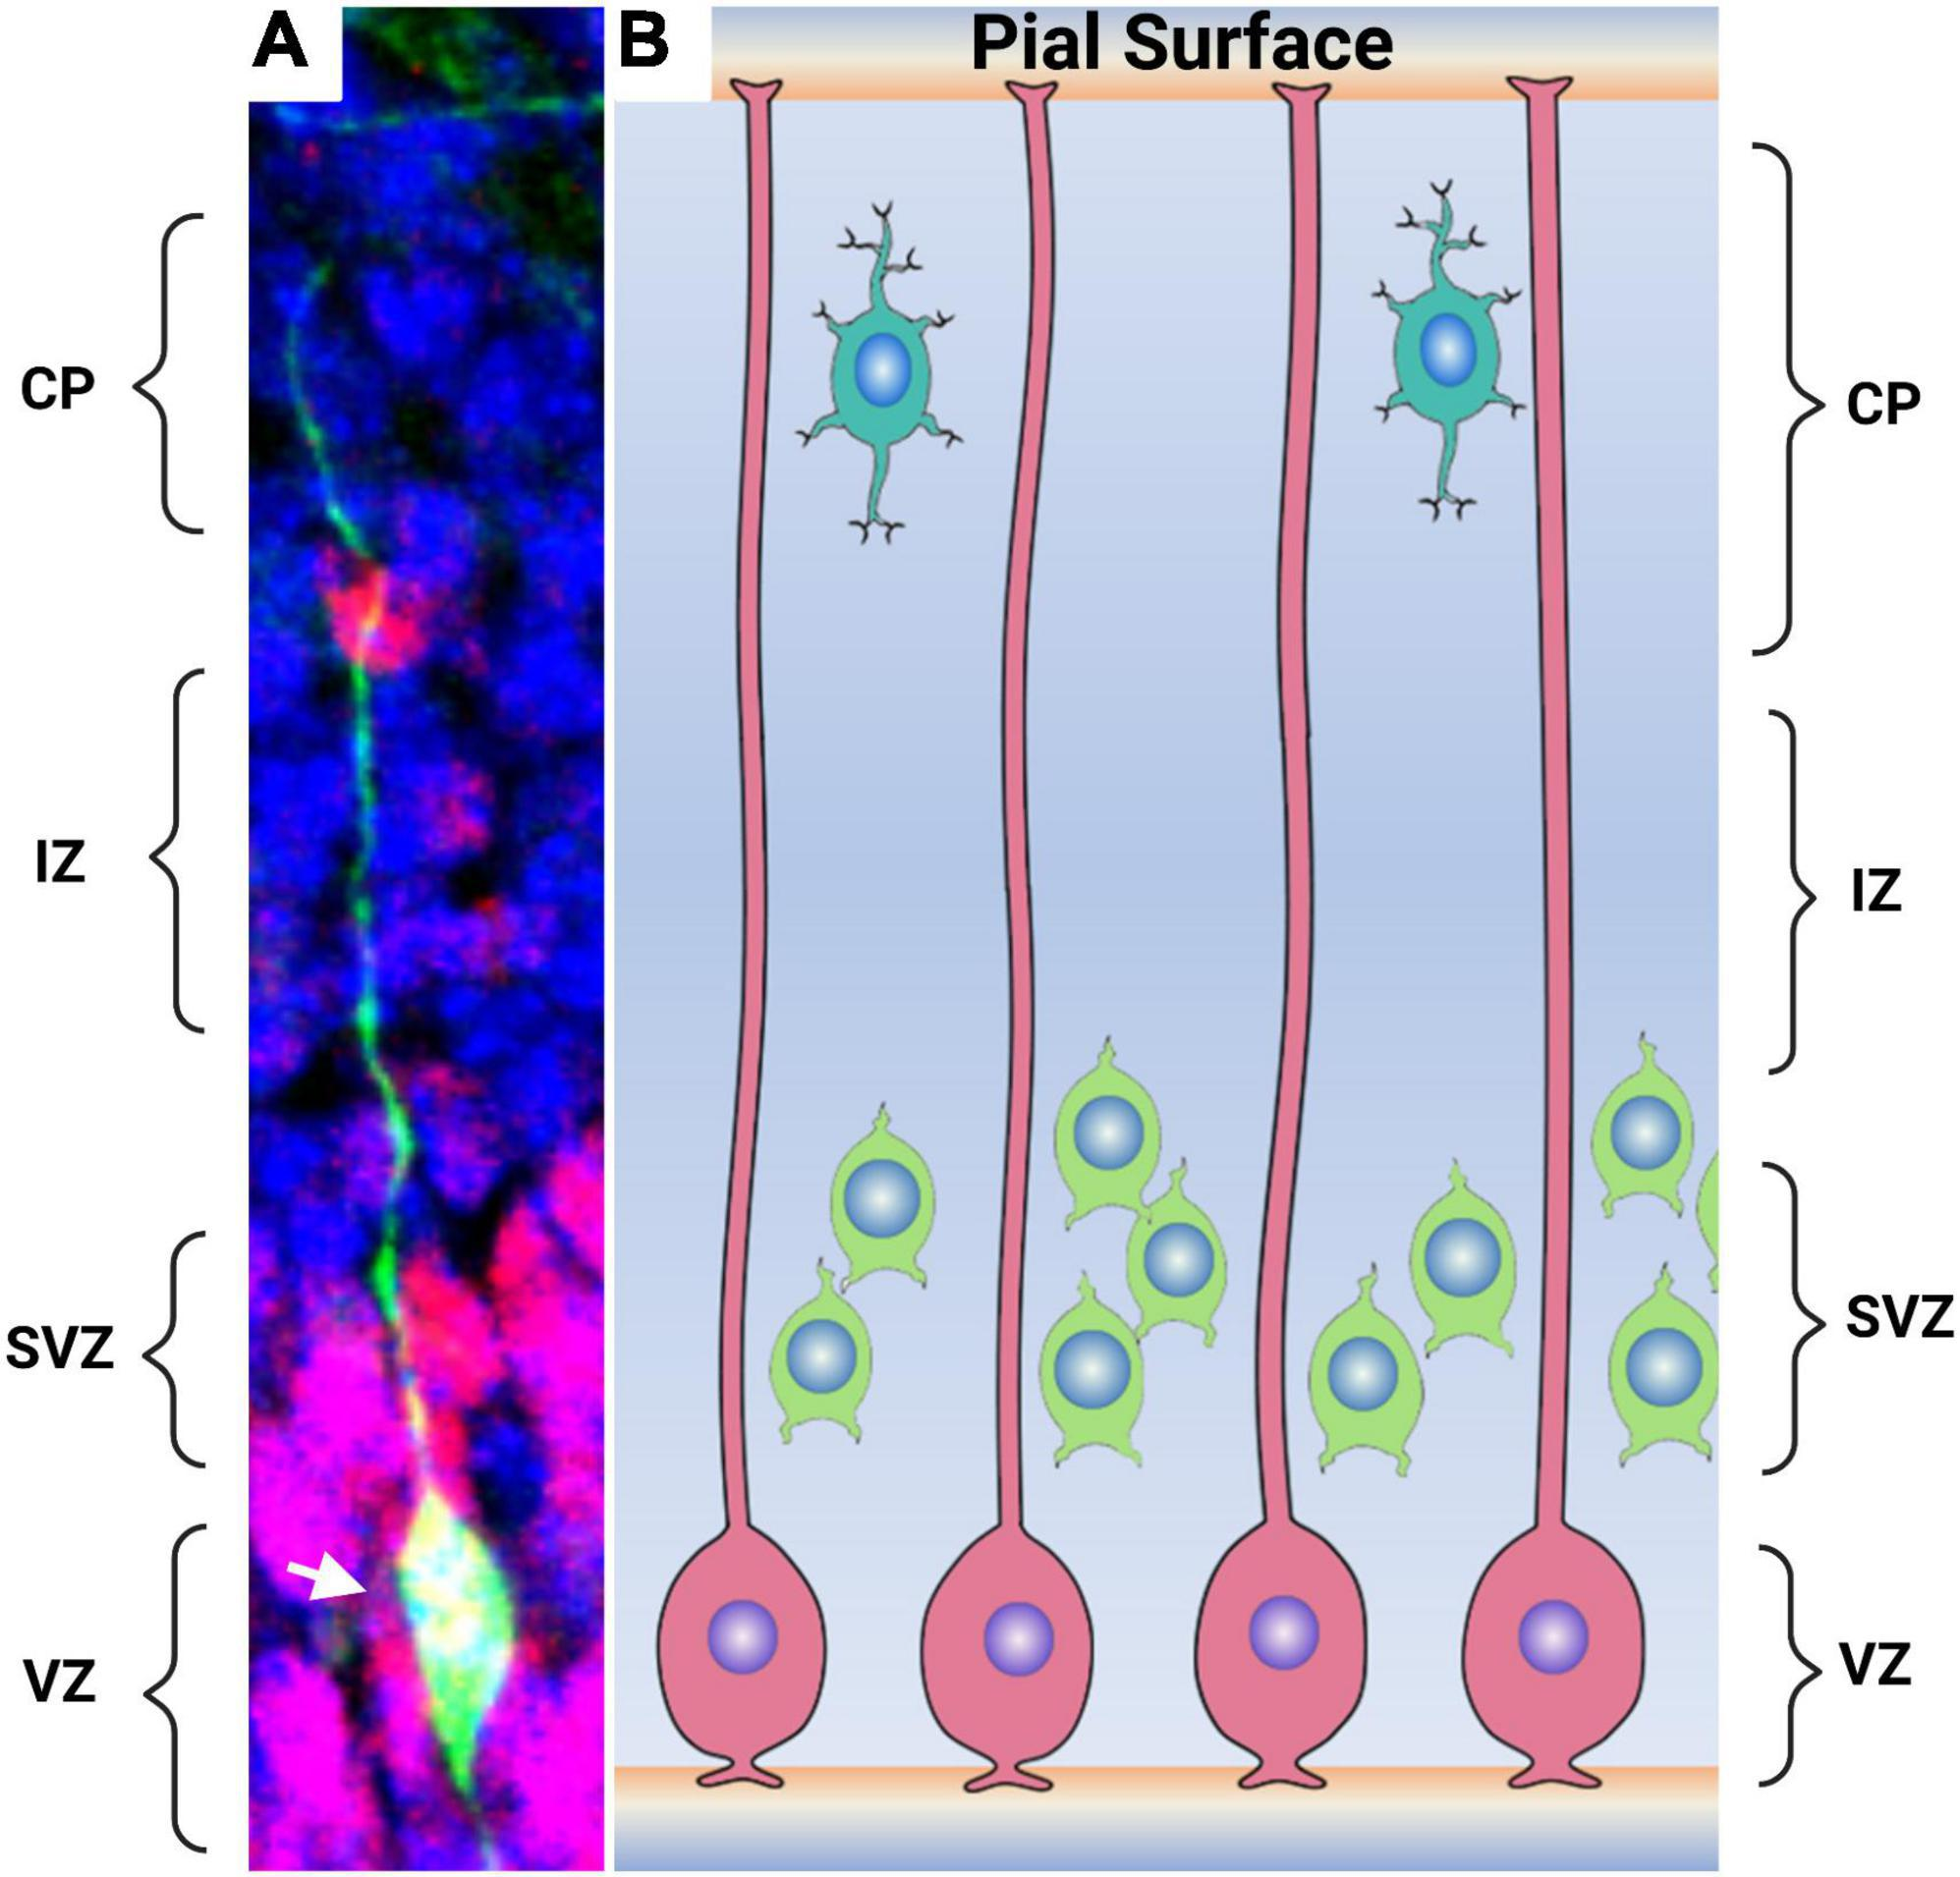
\includegraphics{images/neuro-radialglia.jpg}
\end{itemize}

\hypertarget{cuxe9lulas-de-schwann-e-oligodendruxf3citos}{%
\subsubsection*{Células de Schwann e oligodendrócitos}\label{cuxe9lulas-de-schwann-e-oligodendruxf3citos}}
\addcontentsline{toc}{subsubsection}{Células de Schwann e oligodendrócitos}

Esses tipos celulares são responsáveis por garantir uma condução mais eficiente e célere de impulsos elétricos através dos axônios neuronais por meio da \textbf{mielinização de fibras nervosas}, processo que possibilita a condução saltatória dos potenciais de ação por meio dos nós de Ranvier, pequenos intervalos de membrana desnuda interpostos entre as bainhas de mielina, áreas de revestimento lipídico eletrodinamicamente isolante. Essas células costumam apresentar poucas ramificações (conforme já se pode antever pela própria etimologia grega da palavra ``oligodendrócito''), as quais são primordiais para a fisiologia da mielinização na medida em que se enrolam repetidamente sobre os axolemas neuronais. Nesse âmbito, é necessário destacar que, ao passo que os \textbf{oligodendrócitos} são exclusivos do Sistema Nervoso Central e são capazes de mielinizarem vários axônios ao mesmo tempo, as \textbf{células de Schwann} podem ser observadas exclusivamente no Sistema Nervoso Periférico e podem mielinizar, cada uma, apenas um curto segmento de um dado axônio.

\begin{itemize}
\tightlist
\item
  fotomicrografias e esquemas mostrando as diferenças entre as células de Schwann e os oligodendrócitos
\end{itemize}

Como resultado desses enrolamentos, essas células gliais formam alguns marcos estruturais idetificáveis por meio da microscopia eletrônica de transmissão e muito úteis para o estudo ultraestrutural das doenças desmielinizantes. Estes correspondem ao \textbf{mesaxônio externo}, uma esprial de \textbf{linhas intraperiódicas} (delimitadas pelo espaço extracelular compreendido entre duas voltas sucessivas do prolongamento mielinizador), uma espiral de \textbf{linhas densas principais} (formadas por uma pequena quantidade de citoplasma dos prolongamentos das células mielinizadoras interposta entre dois folhetos internos da estrutura trilaminar de suas membranas plasmáticas, as quais se encontram quase fundidas) e um \textbf{mesaxônio interno}.

\begin{itemize}
\tightlist
\item
  eletromicrografia mostrando a ultraestrutura da bainha de mielina
\end{itemize}

Cabe ressaltar que o processo de mielinização é absurdamente complexo do ponto de vista da Biologia Celular. Resumidamente, seria possível afirmar que, para que a mielina resultante seja viável, são necessárias junções de conexão e de oclusão homotípicas e heterotípicas, proteínas transmembranares responsáveis por compactarem as diversas camadas da espiral formada pelo enrolamento do axônio nos prolongamentos das células mielinizantes (com especial destaque para a proteína zero de mielina e a proteína proteolipídica) e volumes residuais de citoplasma interrompendo a continuidade das linhas densas principais em alguns pontos, correspondendo às \textbf{incisuras de Schmidt-Lantermann}.

\begin{itemize}
\tightlist
\item
  boxe mostrando as incisuras de Schmidt-Lantermann e explicando hipóteses acerca de suas possíveis funções
\end{itemize}

Sob a óptica da Neuropatologia, tem-se que as principais doenças que afetam o processo de mielinização decorrem ou de autoimunidades contra proteínas nele envolvidas (como no caso da esclerose múltipla e da Síndrome de Guillain-Barré) ou de mutações nos genes que as codificam. Para se exemplificar esse último cenário, poderíamos pensar na doença de Charcot-Marie-Tooth ligada ao cromossomo X, onde há um defeito molecular na conexina 32 presente nas junções de comunicação homotípicas presentes nas céulas de Schwann, e na doença de Charcot-Marie-Tooth dos tipos 1B e 2, situação na qual anomalias na proteína zero de mielina levam a prejuízos na compactação das bainhas lipídicas formadas pelos prolongamentos mielinizantes.

\begin{itemize}
\tightlist
\item
  imagens de estrutura proteica terciária computacional mostrando as proteínas zero de mielina ancorando-se entre dois folhetos de membrana plasmática adjacentes
\end{itemize}

\hypertarget{caso-cluxednico}{%
\section{Caso Clínico}\label{caso-cluxednico}}

\hypertarget{cross}{%
\chapter{Cross-references}\label{cross}}

Cross-references make it easier for your readers to find and link to elements in your book.

\hypertarget{chapters-and-sub-chapters}{%
\section{Chapters and sub-chapters}\label{chapters-and-sub-chapters}}

There are two steps to cross-reference any heading:

\begin{enumerate}
\def\labelenumi{\arabic{enumi}.}
\tightlist
\item
  Label the heading: \texttt{\#\ Hello\ world\ \{\#nice-label\}}.

  \begin{itemize}
  \tightlist
  \item
    Leave the label off if you like the automated heading generated based on your heading title: for example, \texttt{\#\ Hello\ world} = \texttt{\#\ Hello\ world\ \{\#hello-world\}}.
  \item
    To label an un-numbered heading, use: \texttt{\#\ Hello\ world\ \{-\#nice-label\}} or \texttt{\{\#\ Hello\ world\ .unnumbered\}}.
  \end{itemize}
\item
  Next, reference the labeled heading anywhere in the text using \texttt{\textbackslash{}@ref(nice-label)}; for example, please see Chapter \ref{cross}.

  \begin{itemize}
  \tightlist
  \item
    If you prefer text as the link instead of a numbered reference use: \protect\hyperlink{cross}{any text you want can go here}.
  \end{itemize}
\end{enumerate}

\hypertarget{captioned-figures-and-tables}{%
\section{Captioned figures and tables}\label{captioned-figures-and-tables}}

Figures and tables \emph{with captions} can also be cross-referenced from elsewhere in your book using \texttt{\textbackslash{}@ref(fig:chunk-label)} and \texttt{\textbackslash{}@ref(tab:chunk-label)}, respectively.

See Figure \ref{fig:nice-fig}.

\begin{Shaded}
\begin{Highlighting}[]
\FunctionTok{par}\NormalTok{(}\AttributeTok{mar =} \FunctionTok{c}\NormalTok{(}\DecValTok{4}\NormalTok{, }\DecValTok{4}\NormalTok{, .}\DecValTok{1}\NormalTok{, .}\DecValTok{1}\NormalTok{))}
\FunctionTok{plot}\NormalTok{(pressure, }\AttributeTok{type =} \StringTok{\textquotesingle{}b\textquotesingle{}}\NormalTok{, }\AttributeTok{pch =} \DecValTok{19}\NormalTok{)}
\end{Highlighting}
\end{Shaded}

\begin{figure}

{\centering 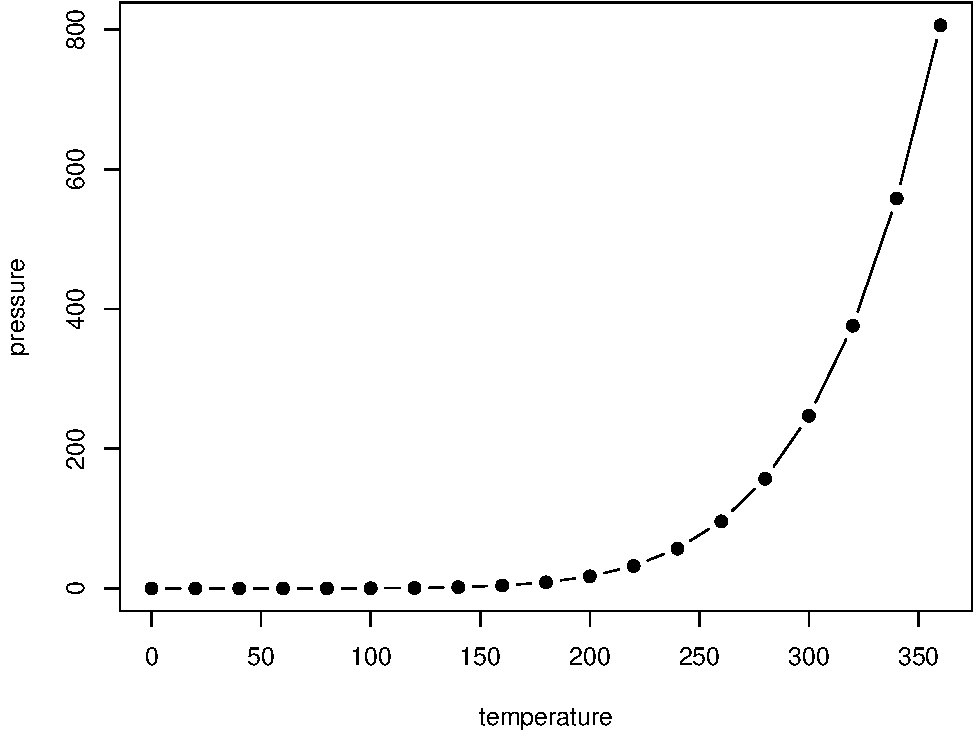
\includegraphics[width=0.8\linewidth]{_main_files/figure-latex/nice-fig-1} 

}

\caption{Here is a nice figure!}\label{fig:nice-fig}
\end{figure}

Don't miss Table \ref{tab:nice-tab}.

\begin{Shaded}
\begin{Highlighting}[]
\NormalTok{knitr}\SpecialCharTok{::}\FunctionTok{kable}\NormalTok{(}
  \FunctionTok{head}\NormalTok{(pressure, }\DecValTok{10}\NormalTok{), }\AttributeTok{caption =} \StringTok{\textquotesingle{}Here is a nice table!\textquotesingle{}}\NormalTok{,}
  \AttributeTok{booktabs =} \ConstantTok{TRUE}
\NormalTok{)}
\end{Highlighting}
\end{Shaded}

\begin{table}

\caption{\label{tab:nice-tab}Here is a nice table!}
\centering
\begin{tabular}[t]{rr}
\toprule
temperature & pressure\\
\midrule
0 & 0.0002\\
20 & 0.0012\\
40 & 0.0060\\
60 & 0.0300\\
80 & 0.0900\\
\addlinespace
100 & 0.2700\\
120 & 0.7500\\
140 & 1.8500\\
160 & 4.2000\\
180 & 8.8000\\
\bottomrule
\end{tabular}
\end{table}

\hypertarget{parts}{%
\chapter{Parts}\label{parts}}

You can add parts to organize one or more book chapters together. Parts can be inserted at the top of an .Rmd file, before the first-level chapter heading in that same file.

Add a numbered part: \texttt{\#\ (PART)\ Act\ one\ \{-\}} (followed by \texttt{\#\ A\ chapter})

Add an unnumbered part: \texttt{\#\ (PART\textbackslash{}*)\ Act\ one\ \{-\}} (followed by \texttt{\#\ A\ chapter})

Add an appendix as a special kind of un-numbered part: \texttt{\#\ (APPENDIX)\ Other\ stuff\ \{-\}} (followed by \texttt{\#\ A\ chapter}). Chapters in an appendix are prepended with letters instead of numbers.

\hypertarget{footnotes-and-citations}{%
\chapter{Footnotes and citations}\label{footnotes-and-citations}}

\hypertarget{footnotes}{%
\section{Footnotes}\label{footnotes}}

Footnotes are put inside the square brackets after a caret \texttt{\^{}{[}{]}}. Like this one \footnote{This is a footnote.}.

\hypertarget{citations}{%
\section{Citations}\label{citations}}

Reference items in your bibliography file(s) using \texttt{@key}.

For example, we are using the \textbf{bookdown} package \citep{R-bookdown} (check out the last code chunk in index.Rmd to see how this citation key was added) in this sample book, which was built on top of R Markdown and \textbf{knitr} \citep{xie2015} (this citation was added manually in an external file book.bib).
Note that the \texttt{.bib} files need to be listed in the index.Rmd with the YAML \texttt{bibliography} key.

The RStudio Visual Markdown Editor can also make it easier to insert citations: \url{https://rstudio.github.io/visual-markdown-editing/\#/citations}

\hypertarget{blocks}{%
\chapter{Blocks}\label{blocks}}

\hypertarget{equations}{%
\section{Equations}\label{equations}}

Here is an equation.

\begin{equation} 
  f\left(k\right) = \binom{n}{k} p^k\left(1-p\right)^{n-k}
  \label{eq:binom}
\end{equation}

You may refer to using \texttt{\textbackslash{}@ref(eq:binom)}, like see Equation \eqref{eq:binom}.

\hypertarget{theorems-and-proofs}{%
\section{Theorems and proofs}\label{theorems-and-proofs}}

Labeled theorems can be referenced in text using \texttt{\textbackslash{}@ref(thm:tri)}, for example, check out this smart theorem \ref{thm:tri}.

\begin{theorem}
\protect\hypertarget{thm:tri}{}\label{thm:tri}For a right triangle, if \(c\) denotes the \emph{length} of the hypotenuse
and \(a\) and \(b\) denote the lengths of the \textbf{other} two sides, we have
\[a^2 + b^2 = c^2\]
\end{theorem}

Read more here \url{https://bookdown.org/yihui/bookdown/markdown-extensions-by-bookdown.html}.

\hypertarget{callout-blocks}{%
\section{Callout blocks}\label{callout-blocks}}

The R Markdown Cookbook provides more help on how to use custom blocks to design your own callouts: \url{https://bookdown.org/yihui/rmarkdown-cookbook/custom-blocks.html}

\hypertarget{sharing-your-book}{%
\chapter{Sharing your book}\label{sharing-your-book}}

\hypertarget{publishing}{%
\section{Publishing}\label{publishing}}

HTML books can be published online, see: \url{https://bookdown.org/yihui/bookdown/publishing.html}

\hypertarget{pages}{%
\section{404 pages}\label{pages}}

By default, users will be directed to a 404 page if they try to access a webpage that cannot be found. If you'd like to customize your 404 page instead of using the default, you may add either a \texttt{\_404.Rmd} or \texttt{\_404.md} file to your project root and use code and/or Markdown syntax.

\hypertarget{metadata-for-sharing}{%
\section{Metadata for sharing}\label{metadata-for-sharing}}

Bookdown HTML books will provide HTML metadata for social sharing on platforms like Twitter, Facebook, and LinkedIn, using information you provide in the \texttt{index.Rmd} YAML. To setup, set the \texttt{url} for your book and the path to your \texttt{cover-image} file. Your book's \texttt{title} and \texttt{description} are also used.

This \texttt{gitbook} uses the same social sharing data across all chapters in your book- all links shared will look the same.

Specify your book's source repository on GitHub using the \texttt{edit} key under the configuration options in the \texttt{\_output.yml} file, which allows users to suggest an edit by linking to a chapter's source file.

Read more about the features of this output format here:

\url{https://pkgs.rstudio.com/bookdown/reference/gitbook.html}

Or use:

\begin{Shaded}
\begin{Highlighting}[]
\NormalTok{?bookdown}\SpecialCharTok{::}\NormalTok{gitbook}
\end{Highlighting}
\end{Shaded}


  \bibliography{book.bib,packages.bib}

\end{document}
